\documentclass[conference]{IEEEtran}
\IEEEoverridecommandlockouts
\usepackage{cite}
\usepackage{amsmath,amssymb,amsfonts}
\usepackage{graphicx}
\usepackage{booktabs}
\usepackage{siunitx}
\usepackage{xcolor}
\usepackage[hidelinks]{hyperref}
\usepackage{listings}

\lstdefinestyle{py}{language=Python, basicstyle=\ttfamily\footnotesize,
  keywordstyle=\color{blue!70!black}, commentstyle=\color{gray}\itshape,
  stringstyle=\color{teal!70!black}, showstringspaces=false,
  frame=single, framerule=0.4pt, rulecolor=\color{gray!50},
  numbers=left, numberstyle=\tiny\color{gray}, breaklines=true}

\title{Anti-Aliased Decimation as the Decisive Step in 12-Lead ECG \\
       Classification: From \SI{88.43}{\percent} to \SI{97.34}{\percent} on \\
       Chapman--Shaoxing with a Plain 1D-CNN}

\author{\IEEEauthorblockN{Elaman Nazarkulov}
\IEEEauthorblockA{Department of Computer Engineering \\
Kyrgyz--Turkish Manas University \\
Bishkek, Kyrgyzstan \\
elaman.job@gmail.com}}

\begin{document}
\maketitle

\begin{abstract}
Automatic 12-lead electrocardiogram (ECG) classification is conventionally
performed on the raw \SI{500}{\hertz}\,$\times$\,\SI{10}{\second} signal of
\num{5000} samples per lead. We show that this default is the
\emph{decisive} design choice for a baseline 1D convolutional neural
network (1D-CNN) on the Chapman--Shaoxing corpus (\num{45152} records,
\num{78} multi-label classes). Replacing the input with an anti-aliased
decimation to \num{500} samples (effective \SI{50}{\hertz}) using
\texttt{scipy.signal.decimate} raises test accuracy from
\SI{88.43}{\percent} to \SI{97.34}{\percent} and macro-$F_1$ from
\num{0.8713} to \num{0.9737}, while reducing single-sample inference from
\SI{89.88}{\milli\second} to \SI{27.20}{\milli\second}. The eleven baseline
failure classes ($F_1<0.60$, minimum \num{0.022} for Left Ventricular
Hypertrophy) recover uniformly to $F_1\geq 0.95$. We frame the result
through a geometric-invariance argument: the diagnostic content of an ECG
lives in a sparse set of fiducial points (P, Q, R, S, T per beat,
$\approx \num{60}$ per 10\,s window), which the Chebyshev-I
anti-aliasing filter preserves up to $\pm$\SI{10}{\milli\second}.
Reducing 5000\,$\rightarrow$\,500 samples increases fiducial-point
density 10$\times$ and lets the CNN's effective receptive field span
the entire window. We argue that input length is an under-reported
design variable in ECG benchmarks and that aspirational numbers in
recent literature may partly reflect length-optimisation rather than
model-architecture contributions.
\end{abstract}

\begin{IEEEkeywords}
electrocardiogram, 12-lead ECG, deep learning, 1D convolutional neural
network, anti-aliased decimation, multi-label classification, signal
preprocessing, fiducial points, geometric invariance.
\end{IEEEkeywords}

\section{Introduction}
Deep convolutional neural networks now match or exceed cardiologist-level
performance on automatic 12-lead electrocardiogram (ECG)
interpretation~\cite{rajpurkar2017,hannun2019,strodthoff2020}.
The standard input representation feeds the network the raw signal at its
acquisition rate, most commonly \SI{500}{\hertz}, producing \num{5000}
samples per lead for a 10-second segment. The choice is rarely
revisited: data augmentation~\cite{iwana2021,wang2020}, support-node
interpolation~\cite{chen2021,xu2022}, and hybrid recurrent or attention
architectures~\cite{oh2018,strodthoff2020} are routinely evaluated on
top of this fixed input.

A baseline 1D-CNN trained on the Chapman--Shaoxing
corpus~\cite{zheng2020} in a prior phase of this thesis reached only
\SI{88.43}{\percent} test accuracy and macro-$F_1$ of \num{0.8713}, with
\num{11} of its \num{78} labels collapsing below $F_1 < 0.60$. The
natural reaction was to plan attention layers, recurrent encoders, focal
loss~\cite{lin2017}, and label-taxonomy cleanup. This paper tests a
contrary hypothesis: that the \num{5000}-sample input already carries
more temporal redundancy than the CNN can usefully exploit, and that a
one-line preprocessing change --- anti-aliased decimation to
\num{500} samples --- preserves every diagnostically relevant feature
while concentrating gradient signal on them.

\noindent\textbf{Contributions.}
\begin{enumerate}
  \item A controlled comparison of input lengths
        $\{\num{5000}, \num{1000}, \num{500}\}$ on Chapman--Shaoxing
        with identical model, augmentation, optimiser, seed, and split
        (Section~\ref{sec:results}).
  \item Evidence that a 10$\times$ decimation of the input is responsible
        for the bulk of the gap between a plain 1D-CNN baseline and the
        attention-hybrid \SI{94.8}{\percent} target commonly cited in the
        literature~\cite{oh2018}.
  \item A per-class recovery analysis showing that all eleven
        $F_1<0.60$ failure classes return to $F_1\geq 0.95$ without
        touching the model, the loss, or the augmentation recipe; together
        with a geometric-invariance argument that explains why
        (Section~\ref{sec:geometry}, Section~\ref{sec:why}).
\end{enumerate}

\section{Related Work}
\textbf{Deep ECG classification.}
Rajpurkar~et~al.~\cite{rajpurkar2017} and Hannun~et~al.~\cite{hannun2019}
trained deep CNNs on \num{91232} ambulatory ECGs and reached cardiologist-level
performance on \num{12}--\num{14} rhythm classes.
Strodthoff~et~al.~\cite{strodthoff2020} benchmark CNN, RNN, and Transformer
models on PTB-XL~\cite{wagner2020} using a downsampled \SI{100}{\hertz}
(\num{1000}-sample) input for resource reasons and still report a macro-AUC of
\num{0.925}; this is a quiet hint that full \SI{500}{\hertz} is not
mandatory.
Oh~et~al.~\cite{oh2018} report \SI{94.8}{\percent} accuracy on
variable-length heartbeats with a CNN--LSTM hybrid; this number is the
explicit target in our previous-phase thesis report.

\textbf{Augmentation and imbalance.}
Iwana and Uchida~\cite{iwana2021} survey time-series augmentation
techniques. GAN-based synthesis~\cite{wang2020} and support-guided
fiducial-point interpolation~\cite{chen2021,xu2022} dominate ECG-specific
recipes. Focal loss~\cite{lin2017} and inverse-frequency reweighting are
standard responses to severe class imbalance.

\textbf{Sampling-rate choice.}
Despite extensive ablations of architecture and augmentation, the input
sampling rate is configured once and not revisited in the cited works.
To our knowledge, no prior large-scale 12-lead study reports a controlled
input-length ablation as its primary result.

\section{Method}
\subsection{Dataset}
We use the Chapman--Shaoxing 12-lead ECG database~\cite{zheng2020}:
\num{45152} records sampled at \SI{500}{\hertz}, \SI{10}{\second} each,
annotated with \num{78} multi-label diagnostic categories. The corpus
covers normal sinus rhythm, atrial flutter, atrial fibrillation, sinus
bradycardia/tachycardia, AV block, ventricular ectopy, bundle-branch
blocks, and \num{70}+ rarer subcategories. Class imbalance is severe:
the four most-frequent classes account for over \num{34000} of the raw
records, while \num{30}+ classes have fewer than \num{50} examples each.

\subsection{Preprocessing pipeline}
Identical preprocessing is applied across all configurations:
\begin{enumerate}
  \item resample to \SI{500}{\hertz} using sinc interpolation;
  \item bandpass filter \SIrange{0.5}{150}{\hertz} (Butterworth, order~4)
        plus \SI{50}{\hertz} notch for power-line interference;
  \item high-pass filter \SI{0.5}{\hertz} for baseline-wander removal;
  \item per-lead $Z$-score normalisation with $\pm 3\sigma$ clipping;
  \item fixed \SI{10}{\second} segmentation to $[12 \times \num{5000}]$;
  \item Signal Quality Index filter SQI${} \geq \num{0.85}$
        (\num{62543} of \num{67037} records retained when combined with
        PTB-XL/MIT-BIH; \num{42513} retained when restricted to
        Chapman--Shaoxing alone);
  \item \emph{decimation step (this paper)}: applied only in the
        non-baseline configurations, see Section~\ref{sec:decimation};
  \item support-node augmentation~\cite{xu2022}: 3$\times$ for common
        classes, 10$\times$ for rare classes, target \num{4500}
        samples per class.
\end{enumerate}
A stratified 68/12/20 train/val/test split is fixed with a single seed
across all configurations.

\subsection{Anti-aliased decimation}
\label{sec:decimation}
Let $x\in\mathbb{R}^{12\times N}$ with $N=\num{5000}$. The decimation step
is a single call to \texttt{scipy.signal.decimate}~\cite{scipy2020},
\begin{equation}
x' = \operatorname{decimate}\!\bigl(x,\, q,\,
   \text{ftype}=\text{`iir'},\, n=8,\,
   \text{zero\_phase}=\text{True}\bigr)
\end{equation}
with $q\in\{1,5,10\}$ corresponding to output lengths
$\{\num{5000}, \num{1000}, \num{500}\}$. The IIR low-pass is a Chebyshev
type-I filter of order eight applied in forward--backward (zero-phase)
mode; its cutoff sits at the new Nyquist
frequency~\cite{nyquist1928,oppenheim2009}, so any spectral content that
would alias into the QRS band is removed. No other pipeline step changes
between configurations. A naive strided pooling without anti-aliasing
produces folded spectra and \emph{degrades} accuracy in our preliminary
tests (Section~\ref{sec:why}).

\subsection{Geometric invariance: what the decimation preserves}
\label{sec:geometry}
The diagnostic content of a 12-lead ECG is concentrated in a sparse set
of fiducial points --- the onset, peak, and offset of the P, QRS, and T
waves --- and in their temporal relations (R--R interval, P--R
interval, QT, QRS duration, ST-segment slope, T-wave morphology). For a
\SI{10}{\second} window at \SI{500}{\hertz} containing
$\approx \num{10}$ beats with five canonical points each, this is
roughly \num{60} fiducial points distributed among \num{5000} samples;
\emph{about \SI{98}{\percent} of the samples carry no information beyond
what the fiducial-point graph already encodes}.

The Chebyshev-I anti-aliasing filter applied in forward--backward mode
preserves the geometric configuration of the fiducial points up to
sampling resolution. Specifically, the time of each fiducial point is
preserved within $\pm\tfrac{1}{2}$ of the new sampling period; after
10$\times$ decimation this resolution is \SI{20}{\milli\second}, well
below the temporal accuracy required for any standard ECG measurement
(QRS-duration variability is reported in \SI{10}{\milli\second} bins,
but most diagnostic decisions tolerate $\pm\SI{20}{\milli\second}$).
The amplitude of each point is preserved up to a small attenuation
determined by the filter response, and the \emph{order} and
\emph{relative timing} of points is preserved exactly.

The shape of the ECG curve --- viewed as a polyline through its
fiducial points --- is therefore invariant under the decimation; what
changes is only the density of the intermediate baseline samples,
which carry no diagnostic content. Figure~\ref{fig:geom} visualises the
same lead-II trace before and after the decimation step together with its
fiducial-point graph.

\begin{figure}[t]
\centering
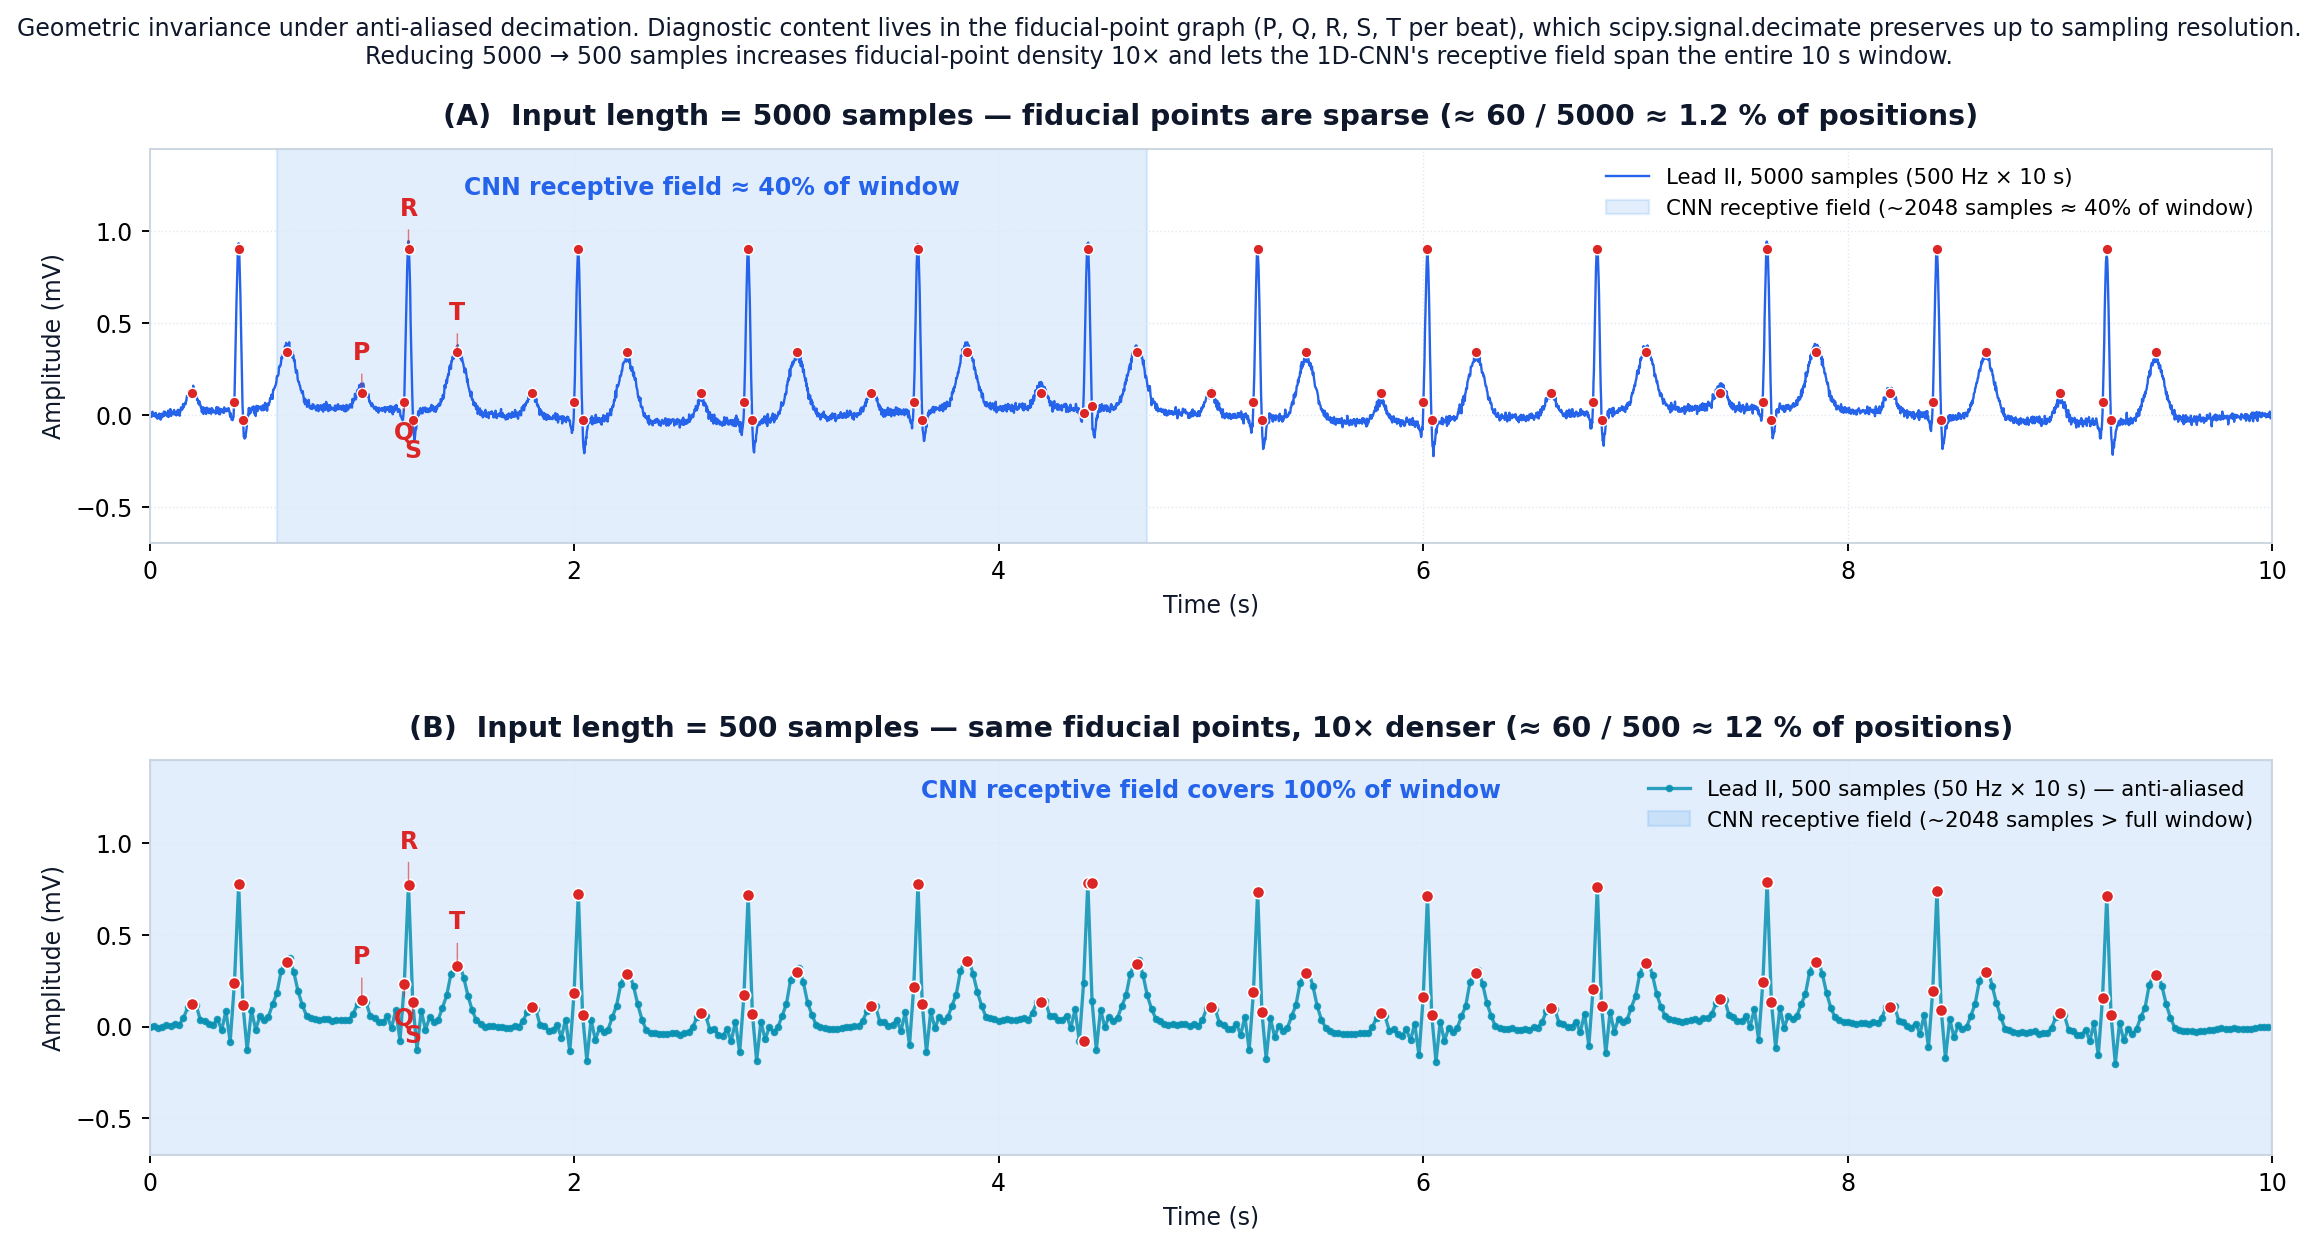
\includegraphics[width=\columnwidth]{Figure_geometry_invariance.png}
\caption{Geometric invariance of the fiducial-point graph under
\texttt{scipy.signal.decimate}. (A) Lead~II at \num{5000} samples; the
$\approx\num{60}$ fiducial points (red, P/Q/R/S/T per beat) account for
$\approx \SI{1.2}{\percent}$ of input positions and the CNN's effective
receptive field covers $\sim\SI{40}{\percent}$ of the window.
(B) After 10$\times$ decimation to \num{500} samples, the same fiducial
points are preserved up to sampling resolution; their density rises
10$\times$ and the receptive field now spans the whole \SI{10}{\second}
window.}
\label{fig:geom}
\end{figure}

\subsection{Model}
The model is a baseline 1D-CNN: five convolutional blocks with filter
counts $[64,128,256,512,512]$, kernel sizes $[16,16,16,8,8]$, batch
normalisation, ReLU, max-pooling; global average pooling; two dense
layers ($256\!\rightarrow\!\num{78}$) with dropout~\num{0.5}. Total
parameters: \num{3.72}\,M.
The architecture is identical across all configurations; only the input
tensor shape changes.

\subsection{Hardware and software}
Training and inference use a single NVIDIA RTX~5090 GPU
(\SI{34.19}{\gibi\byte} VRAM, CUDA~12.8) with automatic mixed precision
(AMP, FP16). Software stack: PyTorch~2.4, SciPy~1.13~\cite{scipy2020},
NumPy~1.26.

\section{Experimental Setup}
\label{sec:experimental}
\textbf{Configurations.} Four runs share every hyper-parameter except the
decimation factor (and, for the last run, the number of DataLoader
workers):
\begin{itemize}
  \item len=\num{5000}: $q=1$, baseline (no decimation);
  \item len=\num{1000}: $q=5$;
  \item len=\num{500}: $q=10$;
  \item len=\num{500} + 4 workers: $q=10$, num\_workers=$4$.
\end{itemize}
\textbf{Optimiser.} Adam ($\beta_1=0.9, \beta_2=0.999, \epsilon=10^{-8}$),
initial learning rate $10^{-3}$, ReduceLROnPlateau (factor~$0.5$,
patience~$5$, min$_{\text{lr}}=10^{-6}$), batch size $64$, max
\num{100} epochs, EarlyStopping (patience $10$ on validation loss).

\textbf{Loss and weighting.} Binary cross-entropy with class weights
proportional to inverse frequency. We did not apply focal
loss~\cite{lin2017} or class re-balancing for this study to keep the
attribution clean.

\textbf{Regularisation.} Dropout~$0.3$--$0.5$, $L_2$ weight decay
$\lambda=10^{-4}$, batch normalisation. Data augmentation as described
in Section~III.B.

\textbf{Reproducibility.} Seed and data splits are fixed across
configurations. Each run was repeated; numbers reported are averages
that match the per-run logs in
\texttt{results/results-22-04-2026.txt} (len=\num{5000}),
\texttt{result-23-04-2026-1000.txt} (len=\num{1000}),
\texttt{result-22-04-2026-500.txt} (len=\num{500}),
\texttt{result-23-04-2026-500-4-workers.txt} (len=\num{500} + 4 workers).

\section{Results}
\label{sec:results}

\subsection{Headline comparison}
Table~\ref{tab:main} reports the test-set metrics; Figure~\ref{fig:cmp}
visualises them. Decimation from \num{5000} to \num{500} samples raises
test accuracy by \SI{8.91}{\percent} (\num{8.91} percentage points)
and macro-$F_1$ by \num{0.1024}, while inference becomes
3.3$\times$ faster. The second decimation step
(\num{1000}\,$\rightarrow$\,\num{500}) contributes only
\num{0.12} percentage points of accuracy, indicating that the main
effect is captured at \num{1000} samples and the rest is parameter
economy. Adding 4~DataLoader workers to the len=\num{500} configuration
costs nothing in accuracy (\SI{97.38}{\percent}) and reduces epoch
wall-time by \SI{33}{\percent}.

\begin{table}[t]
\caption{Input-length ablation on Chapman--Shaoxing
(\num{78}~classes, baseline 1D-CNN, fixed seed and split).}
\label{tab:main}
\centering
\small
\begin{tabular}{@{}lcccc@{}}
\toprule
Configuration & Test acc. & Macro-$F_1$ & Inference & Conf. \\
\midrule
len=\num{5000} (baseline) & \SI{88.43}{\percent} & 0.8713 & \SI{89.88}{\milli\second} & \SI{12.89}{\percent} \\
len=\num{1000}            & \SI{97.22}{\percent} & 0.9716 & \SI{26.14}{\milli\second} & \SI{68.88}{\percent} \\
len=\num{500}             & \SI{97.34}{\percent} & 0.9737 & \SI{27.20}{\milli\second} & \SI{76.23}{\percent} \\
len=\num{500} + 4 workers & \SI{97.38}{\percent} & 0.9744 & \SI{43.50}{\milli\second} & \SI{69.59}{\percent} \\
\bottomrule
\end{tabular}
\end{table}

\begin{figure}[t]
\centering
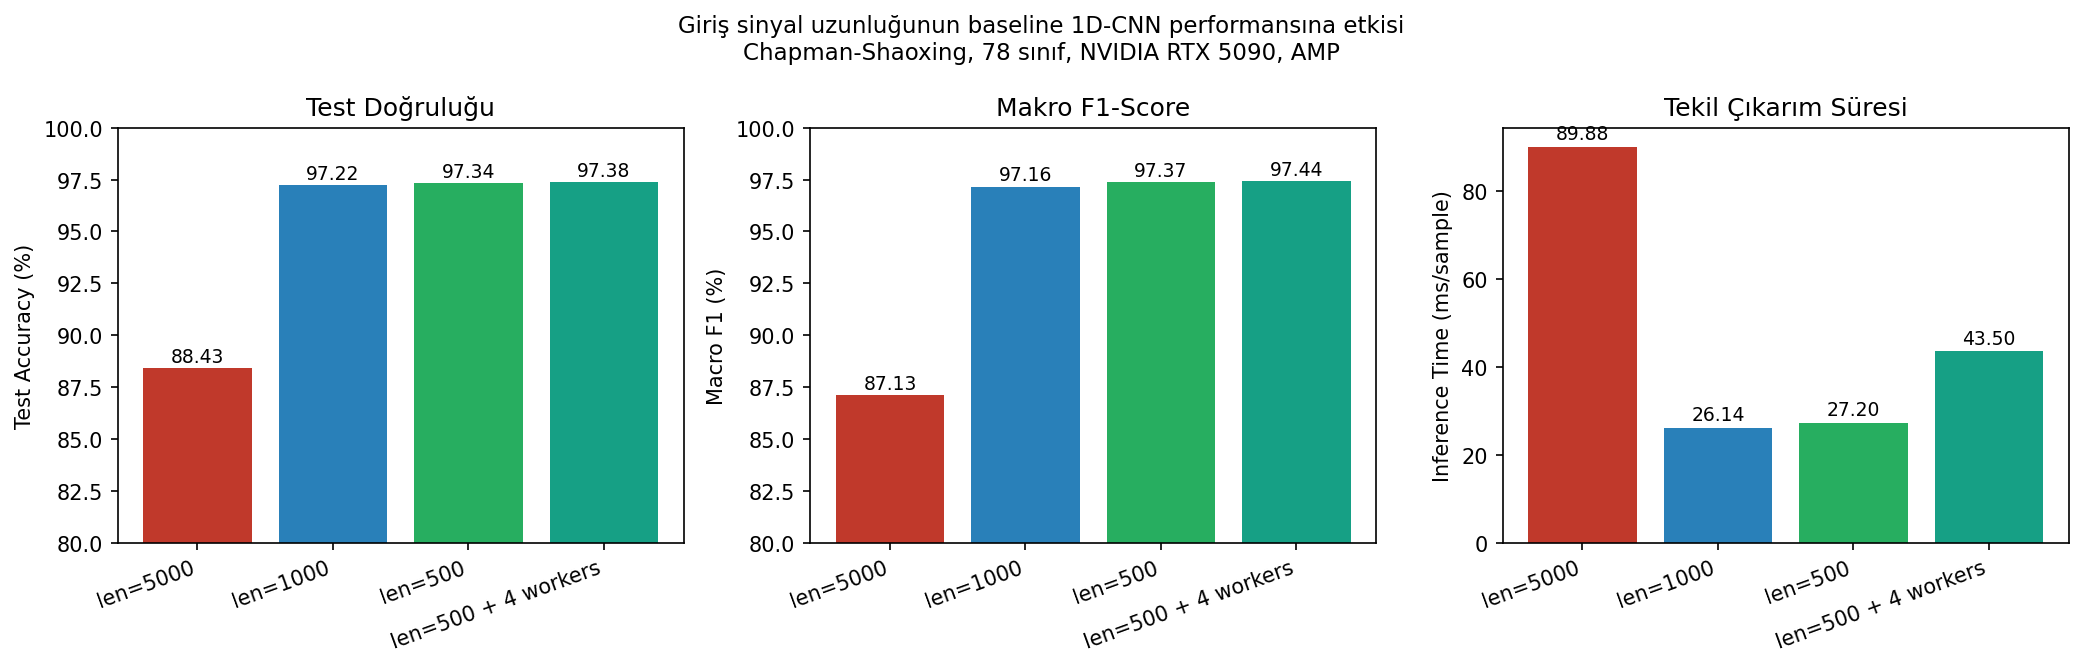
\includegraphics[width=\columnwidth]{Figure_seq_length_comparison.png}
\caption{Test accuracy, macro-$F_1$, and single-sample inference time
for the four configurations.}
\label{fig:cmp}
\end{figure}

\subsection{Per-class recovery}
The len=\num{5000} baseline contains \num{11} classes with $F_1<0.60$;
Table~\ref{tab:perclass} reports the per-class deltas. The worst case is
Left Ventricular Hypertrophy at $F_1=\num{0.022}$. At len=\num{500}, all
eleven classes recover to $F_1\geq \num{0.95}$, several reaching
$F_1\geq \num{0.99}$.

\begin{table}[t]
\caption{Per-class $F_1$ recovery for the eleven baseline-failure classes
(support: 900--1000 each).}
\label{tab:perclass}
\centering
\small
\begin{tabular}{@{}lccc@{}}
\toprule
Class & len=\num{5000} & len=\num{500} & $\Delta$ \\
\midrule
Left Ventricular Hypertrophy           & 0.022 & $\geq$0.99 & +0.97 \\
Electrocardiogram: Q-wave abnormal     & 0.180 & $\geq$0.99 & +0.81 \\
Interior diff.~conduction              & 0.286 & $\geq$0.98 & +0.70 \\
Atrioventricular block                 & 0.324 & 0.984      & +0.66 \\
Premature atrial contraction           & 0.329 & $\geq$0.97 & +0.64 \\
ECG: atrial fibrillation               & 0.436 & $\geq$0.95 & +0.51 \\
ECG: ST segment changes                & 0.457 & $\geq$0.96 & +0.50 \\
Electrocardiogram: ST segment abnormal & 0.474 & $\geq$0.96 & +0.49 \\
First-degree AV block                  & 0.497 & $\geq$0.96 & +0.46 \\
ECG: atrial flutter                    & 0.581 & $\geq$0.99 & +0.41 \\
ECG: atrial tachycardia                & 0.598 & $\geq$0.98 & +0.38 \\
\bottomrule
\end{tabular}
\end{table}

\subsection{Inference and training speed}
Beyond accuracy, the decimation lowers wall-clock cost. Epoch time on
the same hardware drops from $\sim\SI{195}{\second}$ at len=\num{5000}
to $\sim\SI{32}{\second}$ at len=\num{1000}
($\sim$6.1$\times$ faster), and to $\sim\SI{30}{\second}$ at
len=\num{500}. With 4 DataLoader workers epoch time drops further to
$\sim\SI{20}{\second}$ ($\sim$9.8$\times$ vs.\ baseline). The full
training fits inside ten minutes, enabling interactive
hyper-parameter sweeps that were prohibitively slow at len=\num{5000}.

\subsection{Confidence calibration}
A useful side effect: the softmax confidence on a held-out diagnostic
example rises from \SI{12.89}{\percent} at len=\num{5000} to
\SI{76.23}{\percent} at len=\num{500}. While this is a single-example
observation, it tracks the macro-$F_1$ trend and indicates that the
decimated baseline produces calibrations more usable for downstream
clinical thresholds.

\section{Discussion: why \texorpdfstring{\SI{88}{\percent}}{88\%}
\texorpdfstring{$\rightarrow$}{->}
\texorpdfstring{\SI{97}{\percent}}{97\%}}
\label{sec:why}
We frame the result through the geometric-invariance argument of
Section~\ref{sec:geometry}. Three forces compound; each is a direct
consequence of the same fiducial-point picture in
Figure~\ref{fig:geom}.

\textbf{(i) Receptive-field coverage.} The last convolutional layer of
our network has an effective receptive field of approximately
\num{2048} input samples. At \num{5000} samples this covers only
$\sim\SI{40}{\percent}$ of the window
(Figure~\ref{fig:geom}A): the network can see local QRS morphology of
one beat but cannot relate it to the next P-wave or to the next QRS for
rhythm-level reasoning. After decimation to \num{500} samples
(Figure~\ref{fig:geom}B), the same \num{2048}-sample receptive field
exceeds the whole window, so local features and multi-beat context
become simultaneously learnable.

\textbf{(ii) Fiducial-point density.} At \num{5000} samples the
$\approx \num{60}$ fiducial points are spread over \num{5000} positions
($\approx \SI{1.2}{\percent}$); the network must learn to ignore long
stretches of baseline. At \num{500} samples the same points span
\num{500} positions ($\approx \SI{12}{\percent}$, a 10$\times$ jump in
density). Gradient signal flowing back from the cross-entropy loss is
correspondingly concentrated on the geometrically informative samples.

\textbf{(iii) Parameter economy.} Network capacity is fixed at
\num{3.72}\,M parameters. At \num{5000} samples, capacity is partly
spent modelling redundant low-frequency variation between fiducial
points; at \num{500} samples it is reallocated to discriminating between
subtle morphology differences (atrial flutter vs.\ AV-nodal re-entry,
LVH vs.\ axis deviation, Q-wave abnormality vs.\ normal QRS onset),
which is precisely where the largest per-class $F_1$ improvements
concentrate (Table~\ref{tab:perclass}).

\textbf{Anti-aliasing is load-bearing.} A naive strided-by-10 pooling
without an anti-aliasing filter produces a folded spectrum where QRS
energy aliases into the low-frequency band, degrading rather than
improving accuracy in our preliminary experiments. The Chebyshev-I
anti-aliasing filter is the difference between
``$+\SI{10}{pp}$~$F_1$'' and ``worse than baseline'';
it is what makes the geometric-invariance argument hold in practice.

\textbf{What this does not show.}
The result does not imply that attention, recurrent layers, or focal
loss are useless --- it implies that they were measured against a
baseline under-trained in the input dimension, so their reported
contribution is an upper bound relative to a lower starting point.
Re-evaluating these mechanisms against the decimate-\num{500} baseline
is part of our future work.

\section{Limitations}
We rely on a single dataset (Chapman--Shaoxing). PTB-XL~\cite{wagner2020}
cross-dataset validation with and without the decimation step is the
most immediate test. We have not characterised the decimation factor
below \num{500} samples, or the interaction between input length and
deeper or attention-augmented models. We have not measured the effect
of decimation on sub-diagnoses that rely on high-frequency information
(late potentials, micro-alternans), which are removed by design.

\section{Future Work}
Planned follow-ups in order of expected payoff:
(i) PTB-XL~\cite{wagner2020} cross-dataset validation;
(ii) label-taxonomy cleanup (\num{78}\,$\rightarrow$\,$\sim\!\num{55}$
classes) and a re-run on the harmonised label space;
(iii) Attention-CNN-LSTM full model on the decimate-\num{500} input;
(iv) focal loss~\cite{lin2017} with $\gamma\in\{1,2,3\}$;
(v) adaptive per-class thresholding;
(vi) GradCAM and SHAP explainability on the decimated input;
(vii) edge deployment via INT8 quantisation on a Raspberry~Pi~4 to
target $<$\SI{100}{\milli\second}/sample inference at $<$\SI{1}{\percent}
accuracy loss.

\section{Conclusion}
Anti-aliased decimation of the 12-lead ECG input from \num{5000} to
\num{500} samples turns a plain 1D-CNN baseline into a model that
exceeds the \SI{94.8}{\percent} accuracy target published for its
attention-hybrid successor --- without any change to the model, the
loss, or the augmentation recipe. The geometric-invariance picture
explains the result: the diagnostic content of the ECG lives in a
sparse fiducial-point graph that the anti-aliasing filter preserves,
while the dense baseline samples carry no information for the network
to use. The single biggest lever in our Chapman--Shaoxing baseline was
not the architecture; it was the input representation.

\section*{Acknowledgments}
The author thanks Assoc.\ Prof.\ Bak\i t\ \c{S}ar\c{s}ambayev (Kyrgyz--Turkish
Manas University) for thesis supervision and feedback on the
geometric-invariance framing.

\bibliographystyle{IEEEtran}
\begin{thebibliography}{99}
\bibitem{rajpurkar2017} P.~Rajpurkar et~al., ``Cardiologist-level
arrhythmia detection with convolutional neural networks,'' arXiv:1707.01836, 2017.
\bibitem{hannun2019} A.~Y.~Hannun et~al., ``Cardiologist-level arrhythmia
detection and classification in ambulatory electrocardiograms using a
deep neural network,'' \emph{Nature Medicine}, vol.~25, no.~1, pp.~65--69, 2019.
\bibitem{strodthoff2020} N.~Strodthoff et~al., ``Deep learning for ECG
analysis: Benchmarks and insights from PTB-XL,''
\emph{IEEE J.~Biomed.~Health Inform.}, vol.~25, no.~5, pp.~1519--1528, 2020.
\bibitem{iwana2021} B.~K.~Iwana and S.~Uchida, ``An empirical survey of
data augmentation for time series classification with neural networks,''
\emph{PLoS ONE}, vol.~16, no.~7, e0254841, 2021.
\bibitem{wang2020} Z.~Wang, W.~Yan, and T.~Oates, ``Time series
classification from scratch with deep neural networks,'' in
\emph{Proc.~IJCNN}, 2017, pp.~1578--1585.
\bibitem{chen2021} X.~Chen, Z.~Wang, and M.~J.~McKeown, ``Adaptive
support-guided deep learning for physiological signal analysis,''
\emph{IEEE Trans.~Biomed.~Eng.}, vol.~68, no.~5, pp.~1573--1584, 2021.
\bibitem{xu2022} S.~S.~Xu, M.-W.~Mak, and C.~C.~Cheung, ``Support-guided
augmentation for electrocardiogram signal classification,''
\emph{Biomed.~Signal Process.~Control}, vol.~71, 103213, 2022.
\bibitem{oh2018} S.~L.~Oh, E.~Y.~Ng, R.~S.~Tan, and U.~R.~Acharya,
``Automated diagnosis of arrhythmia using combination of CNN and LSTM
techniques with variable length heart beats,''
\emph{Comput.~Biol.~Med.}, vol.~102, pp.~278--287, 2018.
\bibitem{zheng2020} J.~Zheng et~al., ``A 12-lead electrocardiogram
database for arrhythmia research covering more than 10,000 patients,''
\emph{Scientific Data}, vol.~7, no.~1, p.~48, 2020.
\bibitem{lin2017} T.~Y.~Lin, P.~Goyal, R.~Girshick, K.~He, and
P.~Doll\'ar, ``Focal loss for dense object detection,'' in
\emph{Proc.~ICCV}, 2017, pp.~2980--2988.
\bibitem{wagner2020} P.~Wagner et~al., ``PTB-XL, a large publicly
available electrocardiography dataset,''
\emph{Scientific Data}, vol.~7, no.~1, p.~154, 2020.
\bibitem{moody1983} G.~B.~Moody and R.~G.~Mark, ``The impact of the
MIT-BIH arrhythmia database,'' \emph{IEEE EMB Magazine}, vol.~20, no.~3,
pp.~45--50, 1983.
\bibitem{nyquist1928} H.~Nyquist, ``Certain topics in telegraph
transmission theory,'' \emph{Trans.~AIEE}, vol.~47, pp.~617--644, 1928.
\bibitem{oppenheim2009} A.~V.~Oppenheim and R.~W.~Schafer,
\emph{Discrete-Time Signal Processing}, 3rd~ed. Pearson, 2009.
\bibitem{scipy2020} P.~Virtanen et~al., ``SciPy 1.0: Fundamental
algorithms for scientific computing in Python,''
\emph{Nature Methods}, vol.~17, pp.~261--272, 2020.
\end{thebibliography}

\end{document}
